% Descripción de lo que es una red convolucional
\subsection{Redes neuronales}
Las redes neuronales \cite{RedesNeuronales}, también conocidas como redes neuronales artificiales (ANN) o redes neuronales simuladas (SNN),
son un subconjunto de machine learning y están en el corazón de los algoritmos del deep learning. Su nombre y estructura están
inspirados por el cerebro humano, imitando la forma en que las neuronas biológicas se señalan entre sí.\\
Las redes neuronales artificiales (ANN) están compuestas por capas de nodos, que contienen una capa de entrada, una o más
capas ocultas, y una capa de salida. Cada nodo, o neurona artificial, se conecta a otro y tiene un peso y un umbral asociados.
Si la salida de cualquier nodo individual está por encima del valor de umbral especificado, dicho nodo se activa, enviando datos
a la siguiente capa de la red. De lo contrario, no se pasan datos a la siguiente capa de la red. En la figura \ref{fig:SRCNN_RedNeuronal}
se muestra la estructura general de una red neuronal.

\begin{figure}[H]
    \centering
    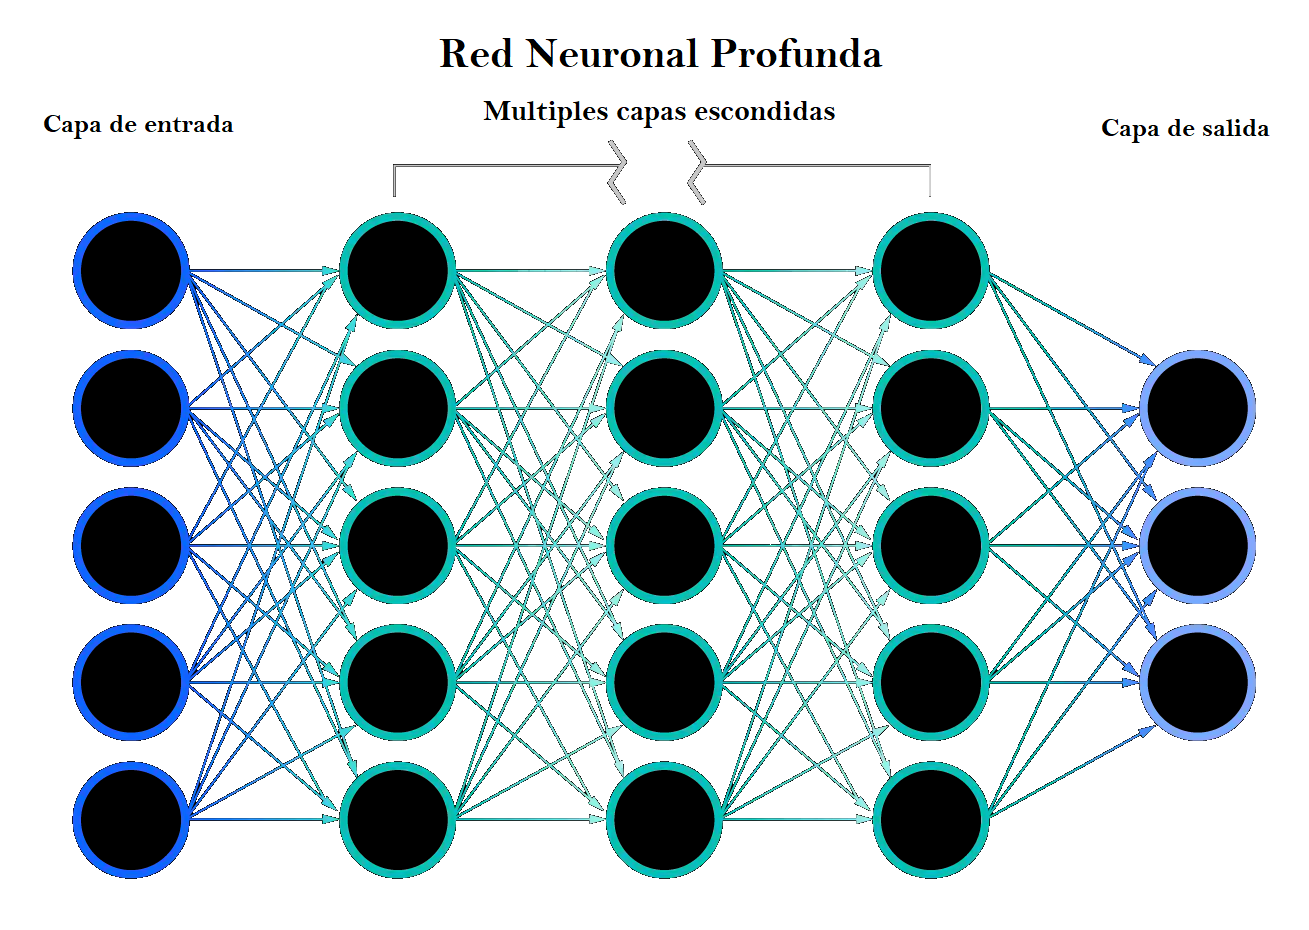
\includegraphics[scale=0.5]{Red_Neuronal.png}
    \caption{Estructura de una red neuronal}
    \label{fig:SRCNN_RedNeuronal}
\end{figure}

Cada nodo o neurona de la red recibe datos de entrada $x_i$ y realiza la suma mediante ponderaciones $w_i$, además de agregar un
sesgo $bias$ y finalmente nos da una salida $f(x)$ solo si $f(x)\geq umbral$, de lo contrario la salida será $0$.

\begin{align}
    \label{eqn:SRCNN_RedNeuronal}
                 x&=\sum_{i=1}^{m}\omega_ix_i+bias
\end{align}
%\begin{align}
%    \nonumber    f(x)&=\left\lbrace\begin{equation}
%                       f(x)\hspace{0.5cm}si\hspace{0.1cm}f(x)>=umbral \\
%                       0\hspace{1.0cm}si\hspace{0.1cm}f(x)<umbral \\
%                    \end{equation}\right.
%\end{align}

\subsection{Redes Convolucionales}
\noindent
Las Redes neuronales convolucionales \cite{RedesConvolucionales} son  un tipo de redes neuronales artificiales  donde las \emph{neuronas}
corresponden a campos receptivos de una manera muy similar a las neuronas en la corteza visual primaria de un cerebro
biológico.  Este tipo de red es una variación de un perceptrón multicapa, sin embargo, debido a que su aplicación es realizada
en matrices bidimensionales, son muy efectivas para tareas de visión artificial, como en la clasificación y segmentación 
de imágenes, entre otras aplicaciones.
Las redes neuronales convolucionales consisten en múltiples capas de filtros convolucionales de una o más dimensiones. Después de
cada capa, por lo general se añade una función para realizar un mapeo causal no-lineal.\\
Como cualquier  red empleada para clasificación, al principio estas redes tienen una  fase de extracción de características,
compuesta de neuronas convolucionales , luego hay una reducción por muestreo y al final tendremos neuronas de perceptrón mas
sencillas para realizar la clasificación final sobre las características extraídas.\\
La fase de extracción de características se asemeja al proceso estimulante en las células de la corteza visual. Esta fase se
compone de capas alternas de neuronas convolucionales y neuronas de reducción de muestreo. Según progresan los datos a lo largo
de esta fase, se disminuye su dimensionalidad, siendo las neuronas en capas lejanas mucho menos sensibles a perturbaciones en
los datos de entrada, pero al mismo tiempo siendo estas activadas por características cada vez más complejas.\\

\subsubsection{Convolucion}
Ahora comienza el \emph{procesado distintivo} de las Redes neuronales convolucionales, es decir, haremos las llamadas
\emph{convoluciones}: Estas consisten en tomar \emph{grupos de pixeles cercanos} de la imagen de entrada e ir operando
matemáticamente (producto escalar) contra una pequeña matriz que se llama kernel.  Ese kernel supongamos que tiene un tamaño
de $3\times 3$ pixels y con ese tamaño logra \emph{visualizar} todas las neuronas de entrada (de izquierda-derecha, de arriba-abajo)
y asi logra generar una nueva matriz de salida, que en definitiva será nuestra nueva capa de neuronas ocultas.\\

\begin{figure}[H]
    \label{fig:SRCNN_Convolucion}
    \centering
    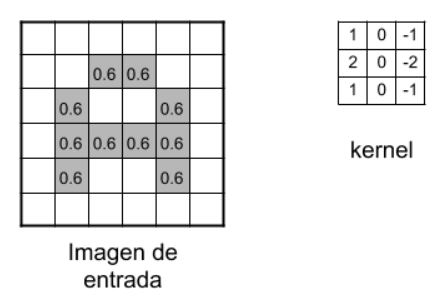
\includegraphics{Convolucion.png}
    \caption{Convolución con \textbf{kernel} de $3\times 3$}
\end{figure}

\subsubsection{Decenso del gradiente}
Para que la red neuronal convolucional \emph{aprenda} se hace uso del algoritmo \emph{backpropagation}, el cual emplea el
algoritmo del descenso del gradiente \cite{DescensoGradiente}, el cual es de uso general y se encarga, de forma numérica, de encontrar un mínimo de
de funciones multivariadas.\\

\begin{figure}[H]
    \label{fig:SRCNN_GradDescent}
    \centering
    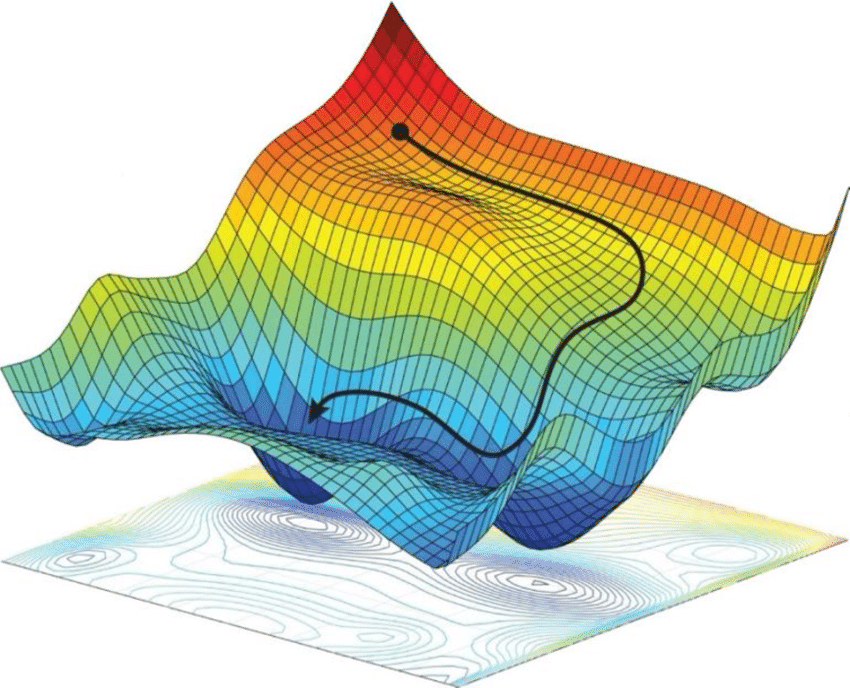
\includegraphics[scale=0.2]{Grad_Des_1.png}
    \caption{Descenso del gradiente}
\end{figure}

Para minimizar la función, podemos seguir el negativo del gradiente, y así ir en la dirección del descenso más pronunciado.
Este es el descenso del gradiente. Formalmente, si comenzamos en un punto $x_0$ y nos movemos una distancia positiva $\alpha$
en la dirección del gradiente negativo, entonces nuestro nuevo y \emph{mejorado} $x_1$ se verá como $x_1=x_0-\alpha\nabla f(x_0)$.
De manera general, podemos definir esto como:

\begin{align}
    \label{eqn:SRCNN_DescensoGradiente}
    x_{n+1}=x_n-\alpha\nabla f(x_n)
\end{align}

\subsubsection{Optimizador Adam (Estimación Adaptiva de Momentos)}
Lo que un optimizador \cite{AdamOptimizador} hace es mejorar los valores de los parámetros de la red con el fin de reducir el error cometido por la red.
Para ello se utiliza (Como se mencionó en el descenso del gradiente) el algoritmo de \emph{backpropagation}.\\
El optimizador más básico posible es actualizar los valores de los parámetros, equitativamente, con base en la \textbf{tasa de
aprendizaje} (\emph{learning rate}), el cual es presentado en \eqref{eqn:SRCNN_DescensoGradiente}, en donde la tasa de aprendizaje
corresponde al parámetro \textbf{$\alpha$} y es un valor constante.\\
El optimizador \textbf{Adam} es un adaptador que pertenece a la familia de \textbf{optimizadores adaptativos}, surge de la
combinación de otros 2 adaptadores pertenecientes a esta familia: \textbf{RMSProp} y \textbf{Momentum}.
El adaptador adam quedá descrito por la siguiente ecuación:

\begin{equation}
    \label{eqn:SRCNN_Adam}
    \begin{split}
        m&=\beta_1m+(1-\beta_1)\nabla W\\
        v&=\beta_2v+(1-\beta_2)\nabla W^2\\
        W&=W-\frac{\alpha m}{\sqrt{v+\epsilon}}
    \end{split}
\end{equation}

Donde en la ecuación \eqref{eqn:SRCNN_Adam} $m$ y $v$ representan los dos momentos, siendo $m$ el que modela la media de los
gradientes a lo largo del tiempo, mientras que $v$ hace lo mismo con la varianza. Por lo general los valores de $\beta_1$ y
$\beta_2$ se fijan como: $\beta_1=0.9$, $\beta_2=0.999$. El parámetro $\alpha$ corresponde a la tasa de aprendizaje y
finalmente $W$ representa los parámetros de la red.

\subsubsection{Error Cuadrático Medio (MSE)}
Mientras entrenamos el modelo, vamos a querer evaluar su precisión usando una función de costo (o pérdida). Esto también
se conoce comúnmente como el error cuadrático medio (MSE). Este se obtiene de la siguiente expresión:

\begin{align}
    \label{eqn:SRCNN_MSE}
    MSE=\frac{1}{2m}\sum_{i=1}^{m}(\hat{y}_i-y_i)^2
\end{align}

Donde en la ecuación \eqref{eqn:SRCNN_MSE}; $i$ representa el indice de la muestra, $\hat{y}$ es el resultado previsto,
$y$ es el valor real y  $m$ es el número de muestras.\\
En última instancia, el objetivo es minimizar nuestra función de costo para asegurar la correción de ajuste para cualquier
observación dada. A medida que el módelo ajusta sus ponderaciones y sesgos, utiliza la función de costo  y el aprendizaje
de refuerzo para alcanzar el punto de convergencia, o el mínimo local. El proceso en el que el algoritmo ajusta sus
ponderaciones es a través del descenso del gradiente (o el optimizador \textbf{Adam}), lo que permite que el módelo
determine la dirección a tomar para reducir los errores (o minimizar la función de costo). Con cada ejemplo de entrenamiento,
los parámetros del módelo se ajustan para converger gradualmente al mínimo.

\begin{figure}[H]
    \label{fig:SRCNN_MSE}
    \centering
    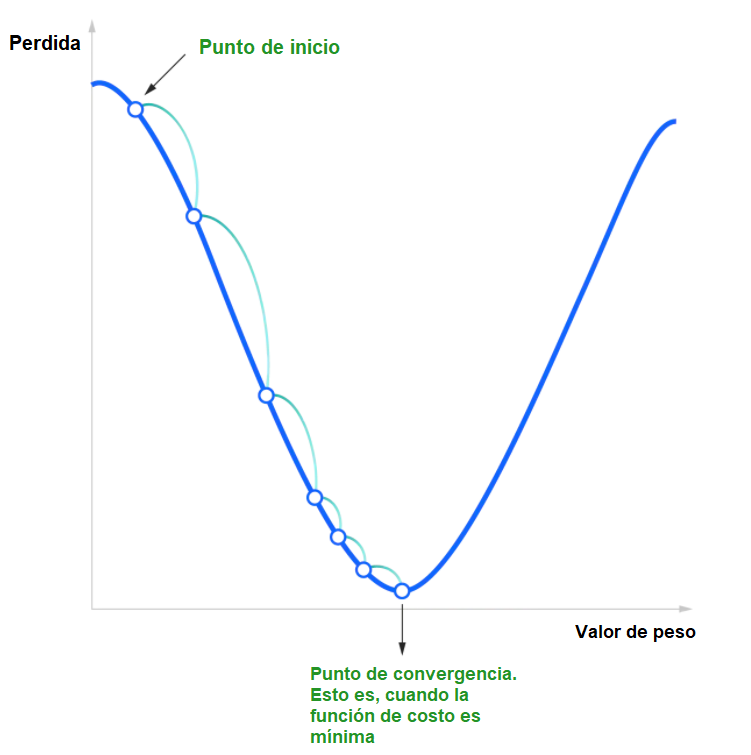
\includegraphics[width=10cm, height=6cm]{MSE.png}
    \caption{Minimización de función de costo (MSE)}
\end{figure}